\documentclass[../main.tex]{subfiles}
\begin{document}

\ifSubfilesClassLoaded{
	\mainmatter
	\setcounter{chapter}{3}
}{}

\chapter{SeaQuest Experiment}
\label{ch:seaquest}

\section{Introduction}
Following the E866 results~\cite{towell2001}, there were great interest in improving
the determination of the light sea-quark asymmetry at large $x$ and to understand
the drop in $\bar{d}/\bar{u}$ at $x>0.25$.
The E906 SeaQuest experiment was proposed as a follow-up to the E866 measurement \cite{isenhower2001}.
The main objective of the experiment is to probe the light sea-quark asymmetry at
large $x$ with better accuracy than previous measurement through the use of the Drell-Yan
process. To gain better statistics at large $x$, the \SI{120}{\GeV} proton beam from the Main
Injector is used instead of the \SI{800}{\GeV} beam from the Tevatron used during E866.
Since the Drell-Yan cross section is inversely proportional to the center-mass energy
squared, the lower beam energy allows for better statistics as large values of $x$.

\section{Beam}
The layout of the Fermilab accelerator complex is shown in \cref{fig:complex},
taken from Ref.~\cite{concept-book}.
SeaQuest received its \SI{120}{\GeV} proton beam from the Fermilab Main Injector.
The proton beam originate from a direct-extraction magnetron hydrogen ion source,
which produces a \SI{35}{\keV} negative hydrogen ion beam. It is then accelerated
to \SI{750}{\keV} using Radio-Frequency Quadrupole. Then the Linac accelerates the
$H^-$ ions to \SI{400}{\MeV}. The $H^-$ ions are then sent through a stripping foil
to remove the electrons. The resulting proton beam then circulates in the Booster
accelerator and accelerates to \SI{8}{\GeV}. The \SI{8}{\GeV} proton beam is
further accelerated by the Main Injector to \SI{120}{\GeV}. The proton beam is
extracted from the Main Injector using a process known as resonant extraction to
provide a lower intensity beam over a 5-second spill, with one spill per minute. The extracted beam, which
is sent to SeaQuest, retains the \SI{53.1}{\MHz} structure of the Main
Injector RF frequency, dividing the beam into ``RF buckets'' that are less than
\SI{2}{\ns} long and occur every \SI{18.8}{\ns}.
\begin{figure}[htbp!]
	\centering
	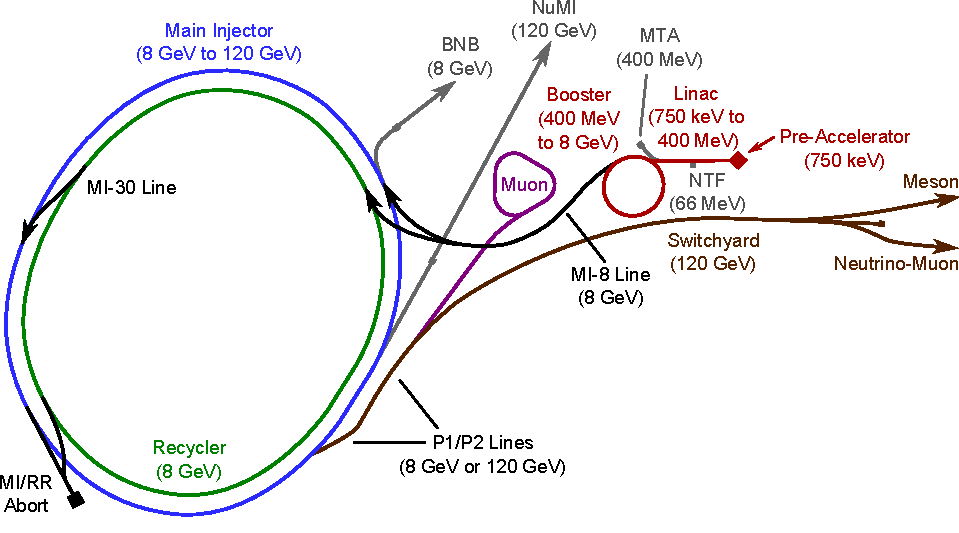
\includegraphics[width=0.6\linewidth]{Fermilab-complex}
	\caption{Layout of the Fermilab accelerator complex, taken from Ref.~\cite{concept-book}. The
		SeaQuest Experimental hall is located on the Neutrino-Muon beamline.}
	\label{fig:complex}
\end{figure}
Even though the integrated intensity from each spill is very stable,
the number of protons in each bucket can vary greatly during the spill, as
is shown in \cref{fig:intensity}.
\begin{figure}[htpb!]
	\centering
	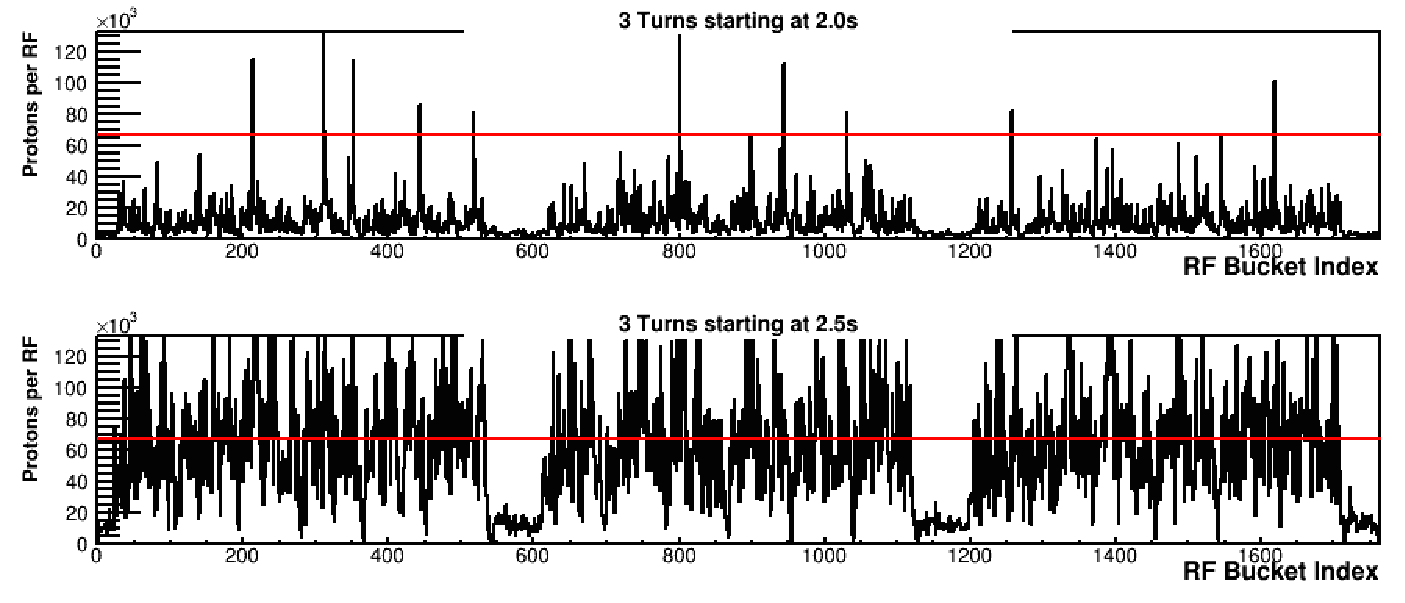
\includegraphics[width =0.8\linewidth]{beam_intensity_v2}
	\caption{The beam intensity measured by the Beam DAQ Cerenkov counter every
		bucket. Taken from Ref.~\cite{aidala2019}}
	\label{fig:intensity}
\end{figure}

\subsection{Beam Intensity Monitor}
\label{subsec:BIM}
The integrated beam intensity is monitor by Fermilab Accelerator Division using a
secondary emission monitor located upstream of the SeaQuest experimental hall.
To better understand the bucket-to-bucket variation in the beam intensity, a Cerenkov counter,
shown in \cref{fig:BIM}, was added upstream of the target during the Main Injector upgrade.
\begin{figure}[htbp!]
	\centering
	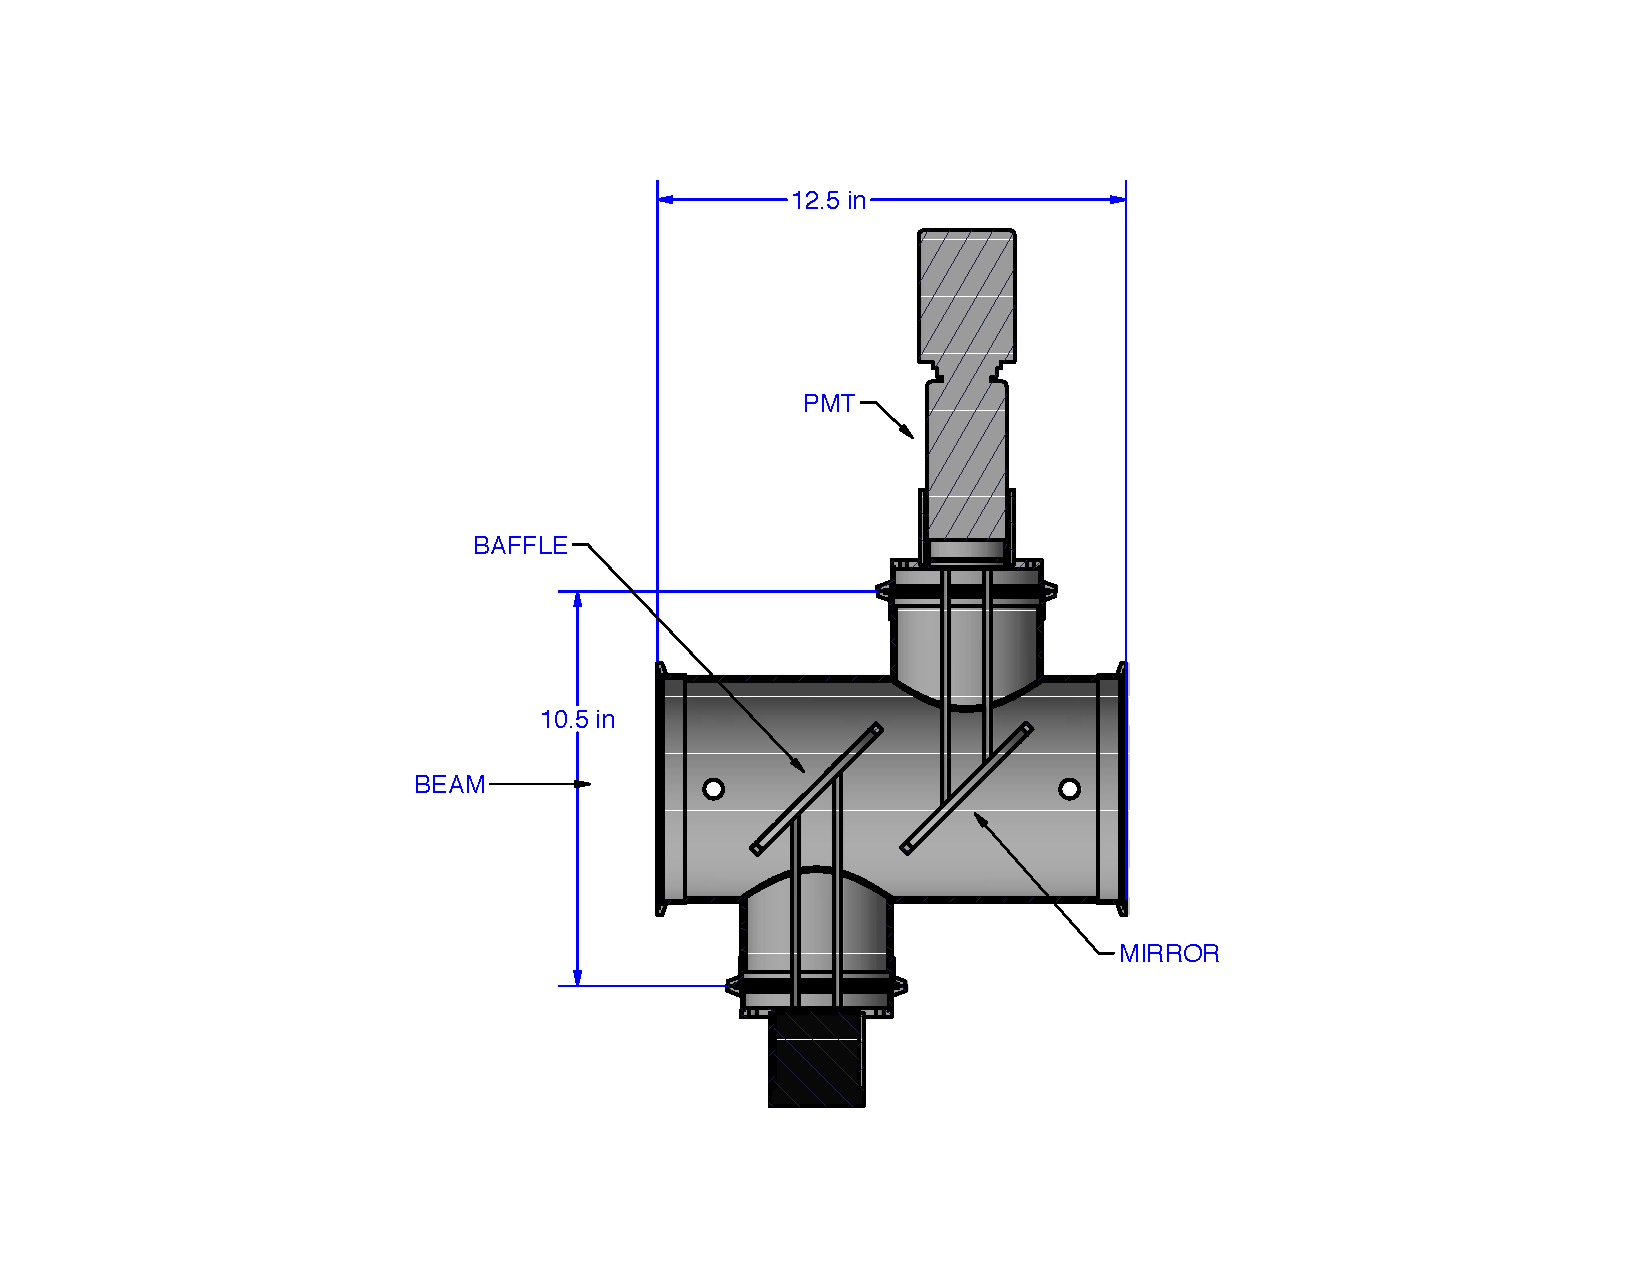
\includegraphics[width=0.4\linewidth]{BIMCerenkov}
	\caption{The Beam Intensity Monitor (BIM) Cerenkov counter. Taken from Ref.\
		\cite{aidala2019}.}
	\label{fig:BIM}
\end{figure}

An aluminized Kapton mirror reflects the Cerenkov light, produced when the proton beam
pass through the radiator, into a single photomultiplier tube. The signal is then
sent to a custom ``QIE'' (Charge Integrator and Encoder) module. This custom module
is clocked with the Main Injector RF, and is capable of recording the beam intensity
of each RF bucket for the entire spill. The QIE module is linked to the trigger
system, and would raise a trigger inhibit when the beam intensity is above a
threshold. The module is also read out by the Beam DAQ, which will be discussed
in \cref{subsec:beamDAQ}. 
The beam intensity monitor is calibrated against a secondary emission monitor.

The ability to record the numbers of proton in each bucket allows us to obtain the
yields as a function of the instantaneous intensity, which will be discussed
further in \cref{M-sec:extrapolation}.

\section{Target}
The SeaQuest target is placed between the Beam Intensity Monitor and the front face
of spectrometer. The target system consists of two liquid targets, hydrogen and deuterium,
and three solid targets, iron, carbon and tungsten. Each solid target is divided
into \num{3} discs of equal length, and are spatially separated along the beam
direction to minimize variation in acceptance between liquid and solid targets.
To account for background originating from the interaction with the instruments,
there are also two calibration targets, an empty vacuum filled flask, known as
empty flask, and the solid target holder, known as no-target. The different targets
are mounted on a motorized table, shown in \cref{fig:target}, which allows the
targets to be interchanged between spills to minimized systematic effect due to
changes in spectrometer performance over time. The properties of the targets and the spills per cycle
of each target positions are listed in \cref{table:target}.
\begin{figure}[htbp!]
	\centering
	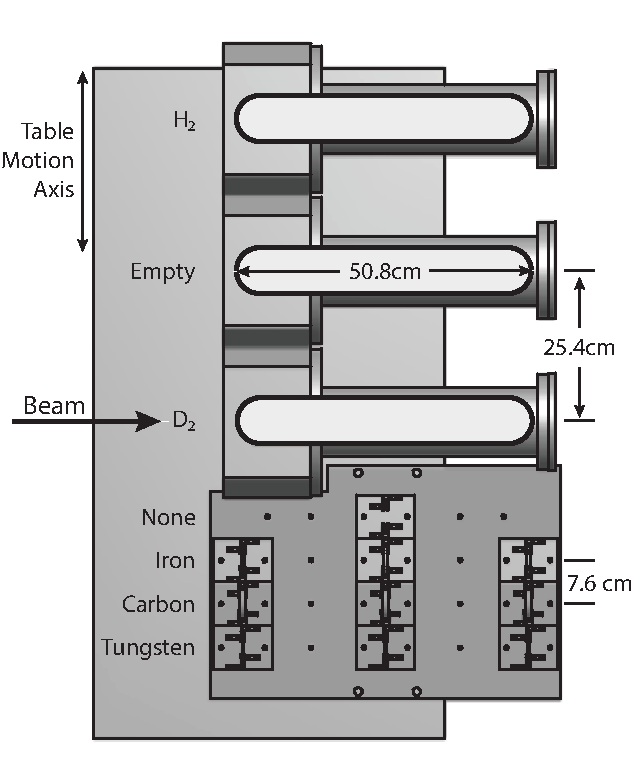
\includegraphics[width=0.4\linewidth]{target-tableLayout}
	\caption{The schematic of the movable target table}
	\label{fig:target}
\end{figure}

\begin{table}[h!]
	\centering
	\caption{SeaQuest target configuration}
	\label{table:target}
	\begin{tabular}{cccccc}
		\hline
		Target      & Position & Density (\unit{\g\per\cm\cubed}) & length (\unit{\cm}) & interaction length   (\unit{\g\per\cm\squared}) & spill/cycle \\ \hline
		\ce{LH_2}   & 1        & \num{0.071}                      & \num{50.8}          & \num{52.0}                                      & 10          \\
		Empty Flask & 2        & -                                & -                   & -                                               & 2           \\
		\ce{LD_2}   & 3        & \num{0.1634}                     & \num{50.8}          & \num{71.8}                                      & 5           \\
		No target   & 4        & -                                & -                   & -                                               & 2           \\
		Iron        & 5        & \num{7.87}                       & \num{1.905}         & \num{132.1}                                     & 1           \\
		Carbon      & 6        & \num{1.80}                       & \num{3.322}         & \num{85.8}                                      & 2           \\
		Tungsten    & 7        & \num{19.30}                      & \num{0.953}         & \num{191.9}                                     & 1           \\
		\hline
	\end{tabular}
\end{table}

\section{Spectrometer and Tracking Station}
The SeaQuest spectrometer consists of two magnets and four tracking stations. A solid iron magnet,
FMag, is placed \SI{104}{\cm} downstream the target. It is then followed by
the first tracking stations. The SeaQuest detector system is separated into four tracking stations.
Stations 1, 2 and 3 each consists of plastic scintillator hodoscopes and drift chambers.
The hodoscopes in each stations provides a fast signal for triggering whereas
the drift chambers provide good spatial resolution for track precise reconstruction.
An open air dipole magnet (KMag) is placed between station 1 and station 2.
Downstream of station 3, there is a 1 m iron wall acting as a
hadron absorber. Station 4 is located behind the hadron absorber and acts as a
muon identifier. Station 4 consists of a hodoscope array and 4 layers of
proportional tube planes.

\begin{figure}[htbp!]
	\centering
	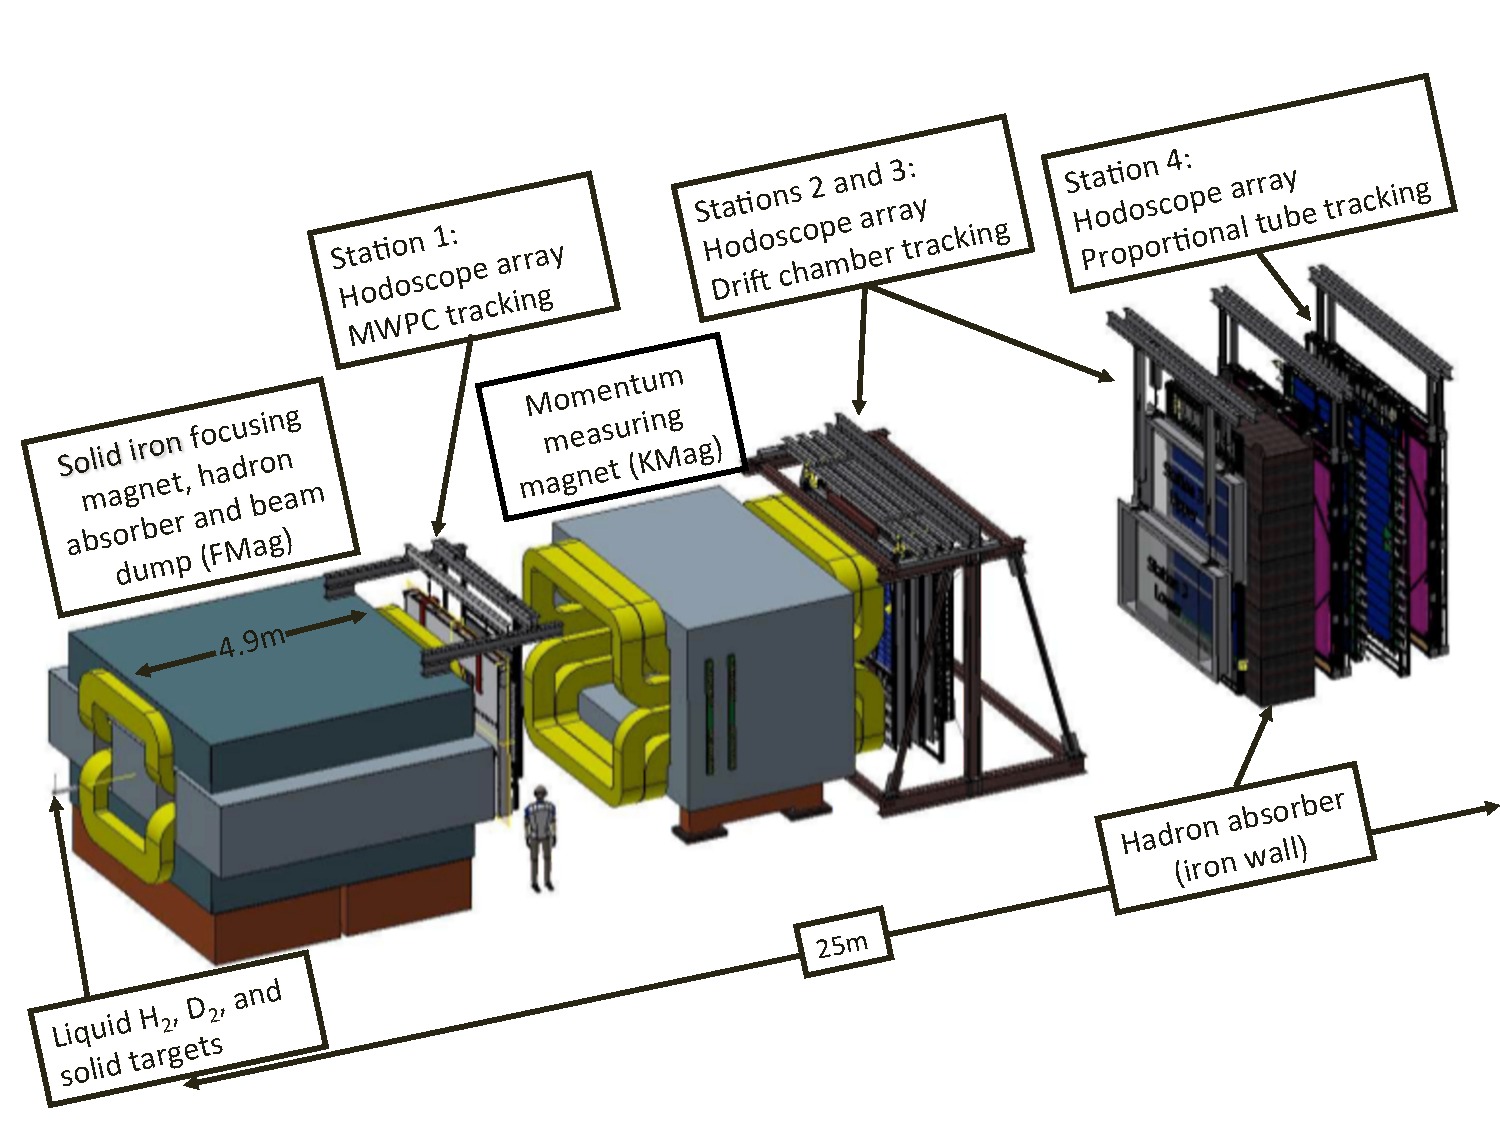
\includegraphics[width=0.6\linewidth]{SeaQuestSpectrometer}
	\caption{schematics of the SeaQuest spectrometer. Taken from Ref.~\cite{aidala2019}}
	\label{fig:spectrometer}
\end{figure}

\subsection{Magnets}
There are two dipole magnets used in the SeaQuest spectrometer, namely the focusing
magnet (FMag) and analyzing magnet (KMag). The magnetic field of both magnets point
in the same direction vertically ($\pm y$), which bend the muons horizontally along
the $x-z$ plane. The polarity of the magnets were flipped during Run 3, partly to reduce
radiation damage to electronics located in the hall.

The upstream focusing magnet (FMag) is a solid iron magnet, shown in \cref{fig:fmag}.
It measures at \SI{503}{\cm} by \SI{302.4}{\cm} tall by \SI{160}{\cm} wide.
The magnet consists of a stack of high purity iron, recovered from
the Columbia University Nevis Laboratory Cyclotron, and the aluminium coils from the E866
SM3 magnet. The coils are excited to \SI{2000}{\ampere} and generate an \SI{1.9}{\tesla}
magnetic field within the iron block. This corresponds to a transverse momentum kick of
\SI{3.07}{\GeV}. FMag serves three main purposes: focusing high mass muon pairs, beam
dump and hadron absorber. As a focusing magnet, FMag would focus dimuons with high $p_T$
or high mass into the spectrometer acceptance. This is particularly important as SeaQuest
aims to probe the partonic structure at high $x$, which would correspond to high mass.
Additionally, it would also defocus the low momentum muons, hence reducing the background.
Due to the high beam intensity, FMag also serves as beam dump. Typically, only $\sim 10\%$
of the proton beam would interact with target material. The remaining protons would interact
within FMag. The hadrons produced during this process would also be absorbed by the iron,
while allowing muons into the spectrometer.
A \SI{5}{\cm} diameter by \SI{25}{\cm} deep hole is drilled into the upstream
end of FMag along the beam axis. This is done to move the initial interaction points
of the beam with the beam dump further away from the targets, allowing for better target/dump
separation. This also reduces the radiation within the target cave, which facilitate the
access to the target area for maintenance.
The magnetic field distribution is modeled using a magnetostatic modeling program. The
excitation is measured by wrapping a 1-turn coil around the central region of the magnet to measure the induced
current. Final calibration of the field strength is determined by the reconstructed
mass of the $J/\psi$ resonance.
\begin{figure}[h!]
	\centering
	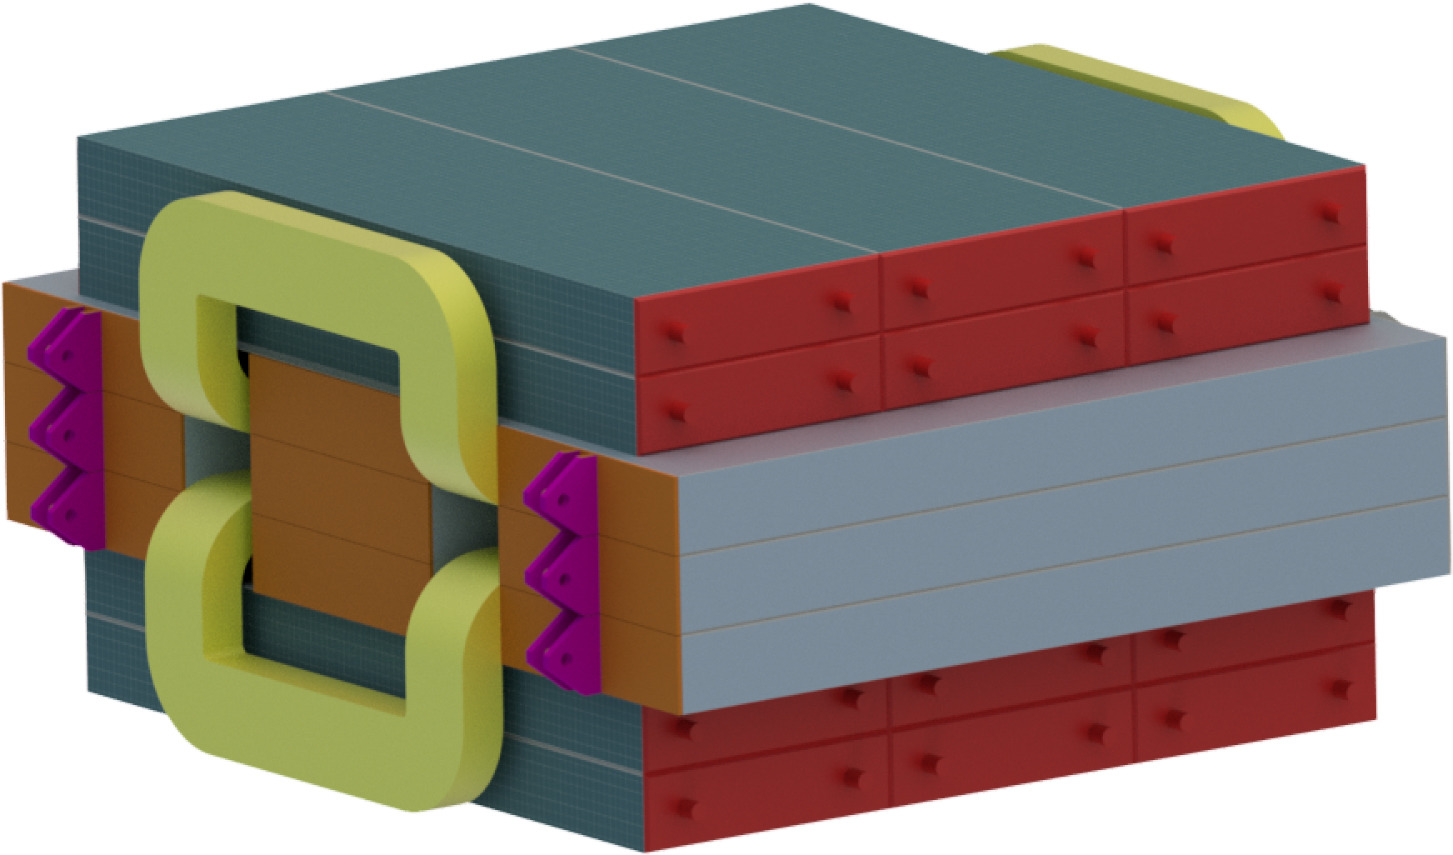
\includegraphics[width=0.5\linewidth]{FMAG}
	\caption{Perspective drawing of FMag showing the arrangement of the iron slabs.
		Taken from Ref.~\cite{aidala2019}.}
	\label{fig:fmag}
\end{figure}

The downstream analyzing magent (KMag) is a \SI{3}{\meter} long open aperture magnet
with a \SI{289}{\cm} wide by \SI{203}{\cm} high central air gap. It was
originally  constructed by E799/KTeV collaboration\cite{alavi-harati2003}.
The coils are excited to \SI{1600}{\ampere} which produce a magnetic field of \SI{0.4}{\tesla},
corresponding to a \SI{0.41}{\GeV} transverse momentum kick. The primary purpose for
KMag is to determine the momentum of the muons. The magnetic field is measured using a Hall
probe and is further calibrated using the reconstructed mass of the $J/\psi$ resonance.


\subsection{Hodoscope}
A hodoscope is placed on upstream end of each tracking stations. Each of the hodoscope planes
is composed of overlapping panels of scintillators viewed by photomultiplier tubes (PMTs) at the end.
When a charged particle pass through the scintillator, the molecules would be excited and
release photons. These photons are then collected at the PMTs, the amplified signals are
then send through discriminators. The signal is then recorded by the Data Acquisition (DAQ) System
using Time-to-Digital converters (TDCs).
The primary purpose of the scintillator hodoscopes is to provide fast signal for the
trigger system. It is also used during reconstruction to reduce the number of chamber hits.
The x-planes are placed vertically to measure the bend plane position.
And the y-planes are arranged horizontally to measure the non-bend plane position.
The scintillator bars in each plane is also split in the middle, denoted as Top and Bottom
for the x-planes, or Left and Right for the y-planes.

Station~1 and 2 each have single x-y planes. Station~3 has a single x plane, and station
4 has two y planes and one x plane. The scintillator bars used in St~.1 and 2 are recycled
from HERMES experiment~\cite{ackerstaff1998a}, whereas new Eljen EJ-200 scintillator material
is used for St.~3 and 4. Because of the physical size of the sintillatior bars in St.~4, the station~4
hodoscopes have PMTs on both ends of the sintillator bars. Each of the PMT base has a
``clip line'' attached at the output to reduce the output pulse from $20-25$\unit{\ns}
down to $10-15$\unit{\ns} full width.

The configuration of the hodoscope is summarized in \cref{table:hodo}. \pdfmargincomment{why are there 2 y hodo in St4? Lower rate at St4? Shivangi's thesis is correct NIM paper is wrong}
\begin{table}[h!]
	\centering
	\caption{SeaQuest hodoscope configuration}
	\label{table:hodo}
	\begin{tabular}{lllllll}
		\hline
		Plane & Number      & Length (\unit{\cm}) & Width (\unit{\cm}) & Thickness (\unit{\cm}) & Array Width (\unit{\cm}) & Location (\unit{\cm})                                                 \\ \hline
		1Y    & $20\times2$ & \num{78.7}          & \num{7.32}         & \num{0.64}             & \num{140}                & \num{667}                                                             \\
		1X    & $23\times2$ & \num{69.9}          & \num{7.32}         & \num{0.64}             & \num{161}                & \num{654}                                                             \\
		2Y    & $19\times2$ & \num{132.0}         & \num{13.0}         & \num{0.64}             & \num{241}                & \num{1402}                                                            \\
		2X    & $16\times2$ & \num{152.0}         & \num{13.0}         & \num{0.64}             & \num{203}                & \num{1421}                                                            \\
		3X    & $16\times2$ & \num{167.6}         & \num{14.6}         & \num{1.3}              & \num{224}                & \num{1958}                                                            \\
		4Y1   & $16\times2$ & \num{152.4}         & \num{23.5}         & \num{1.3}              & \num{366}                & \begin{tabular}[c]{@{}l@{}}\num{2130}(L)\\ \num{2146}(R)\end{tabular} \\
		4Y2   & $16\times2$ & \num{152.4}         & \num{23.5}         & \num{1.3}              & \num{366}                & \begin{tabular}[c]{@{}l@{}}\num{2200}(L)\\ \num{2217}(R)\end{tabular} \\
		4X    & $16\times2$ & \num{182.9}         & \num{19.6}         & \num{1.3}              & \num{305}                & \begin{tabular}[c]{@{}l@{}}\num{2236}(T)\\ \num{2251}(B)\end{tabular} \\
		\hline
	\end{tabular}
\end{table}

\subsection{Drift Chambers}
The resolution of the hodoscope is limited by the physical size of the scintillator bars.
Drift chamber are used to provide a better position resolution of the muons at each station.
A drift chamber measures the position by recording the drift time of the electrons created
by the ionization of the gas mixture when charged particles pass through the chamber.
Each drift chamber consist of six planes of sense wires. The wires in two planes,
denoted as X and X$'$, are aligned vertically. Two planes are tilted by \ang[retain-explicit-plus]{+14},
denoted as U and U$'$, and two planes, V and V$'$, are tilted by \ang[retain-explicit-plus]{-14}.
The wires in the primed planes are offset by half a drift cell relative to the
unprimed planes to resolve left-right ambiguity of the drift direction.
Station 1 and 2 each have one chamber referred as D1 and D2. The chamber at station
3 is separated into top and bottom halves, denoted as D3p and D3m.

In data sets 1-3, a smaller chamber, D1.1, was used. It was later replaced by a newly constructed
chamber, D1.2, with better expected high rate capacity in data set 4-6. However, D1.1 would be
reinstalled later for data set 5-6. D3m.1 was used during the commissioning run, data set 1, and
was later replaced by D3m.2 for the later data sets.

The D1.1, D2 and D3m.1 chambers were recycled from previous Fermilab experiments, E605 (D2 and D3m.1)~\cite{moreno1991}
and E866 (D1.1)~\cite{hawker1998}. The other chambers were designed and constructed for the SeaQuest experiment.
Specifications of each chamber are listed in \cref{table:chamber}.

The signals from the sense wires are fed to ASDQ (Amplification, Shaper, Discriminator and Charger integrator)
cards which are used for amplification and discrimination. The signal is then fed to LSB (Level Shifter Board)
to covert into standard LVDS (low voltage differential signal), which can then be read out by the TDC
modules and recorded by the DAQ system.

\begin{table}[h!]
	\centering
	\caption{SeaQuest drift chamber configuration. The primed planes are almost the same as the unprimed
		planes. The positions of the X planes are defined to be the distance between the chamber and the
		upstream face of FMag, while the positions for U and V denote the offset relative to the corresponding
		X plane.}
	\label{table:chamber}
	\begin{tabular}{cccccc}
		\hline
		Chamber & Plane & \# of wires & Cell width (\unit{\cm}) & Width\texttimes Height (\unit{\cm}\texttimes\unit{\cm}) & z Position (\unit{cm}) \\ \hline
		D1.1    & X     & \num{160}   & \num{0.64}              & $102\times 122$                                         & \num{617}              \\
		        & U, V  & \num{201}   & \num{0.64}              & $101\times 122$                                         & $\pm20$                \\
		D1.2    & X     & \num{320}   & \num{0.50}              & $153\times 137$                                         & \num{691}              \\
		        & U, V  & \num{384}   & \num{0.50}              & $153\times 137$                                         & $\pm1.2$               \\
		D2      & X     & \num{112}   & \num{2.1}               & $233\times264$                                          & \num{1347}             \\
		        & U, V  & \num{128}   & \num{2.0}               & $233\times264$                                          & $\pm25$                \\
		D3p     & X     & \num{116}   & \num{2.0}               & $232\times166$                                          & \num{1931}             \\
		        & U, V  & \num{134}   & \num{2.0}               & $268\times166$                                          & $\pm6$                 \\
		D3m.1   & X     & \num{176}   & \num{1.0}               & $179\times168$                                          & \num{1879}             \\
		        & U, V  & \num{208}   & \num{1.0}               & $171\times163$                                          & $\pm19$                \\
		D3m.2   & X     & \num{116}   & \num{2.0}               & $232\times166$                                          & \num{1895}             \\
		        & U, V  & \num{134}   & \num{2.0}               & $268\times166$                                          & $\pm6$                 \\ \hline
	\end{tabular}
\end{table}

\subsection{Proportional tubes}
The muon identification is accomplished with the proportional tube at station 4. A \SI{1}{\meter} thick
iron wall separate station 3 and 4, which acts as an absorber to stop hadrons and electrons from reaching
station 4. For precise track reconstruction, there are four layers of proportional tubes planes. Each plane
is made of eight proportional tube modules, with 16 proportional tubes per module. The 16 proportional tubes
in each module further divided into two sub-layers, with the second layers shifted by half a tube width to
resolve the left-right ambiguity, as in the case of drift chambers. The proportional tubes oriented horizontally
(vertically) are in the first and fourth (second and third) planes as shown in \cref{fig:prop}
\begin{figure}[ht!]
	\centering
	\begin{subfigure}{0.45\linewidth}
		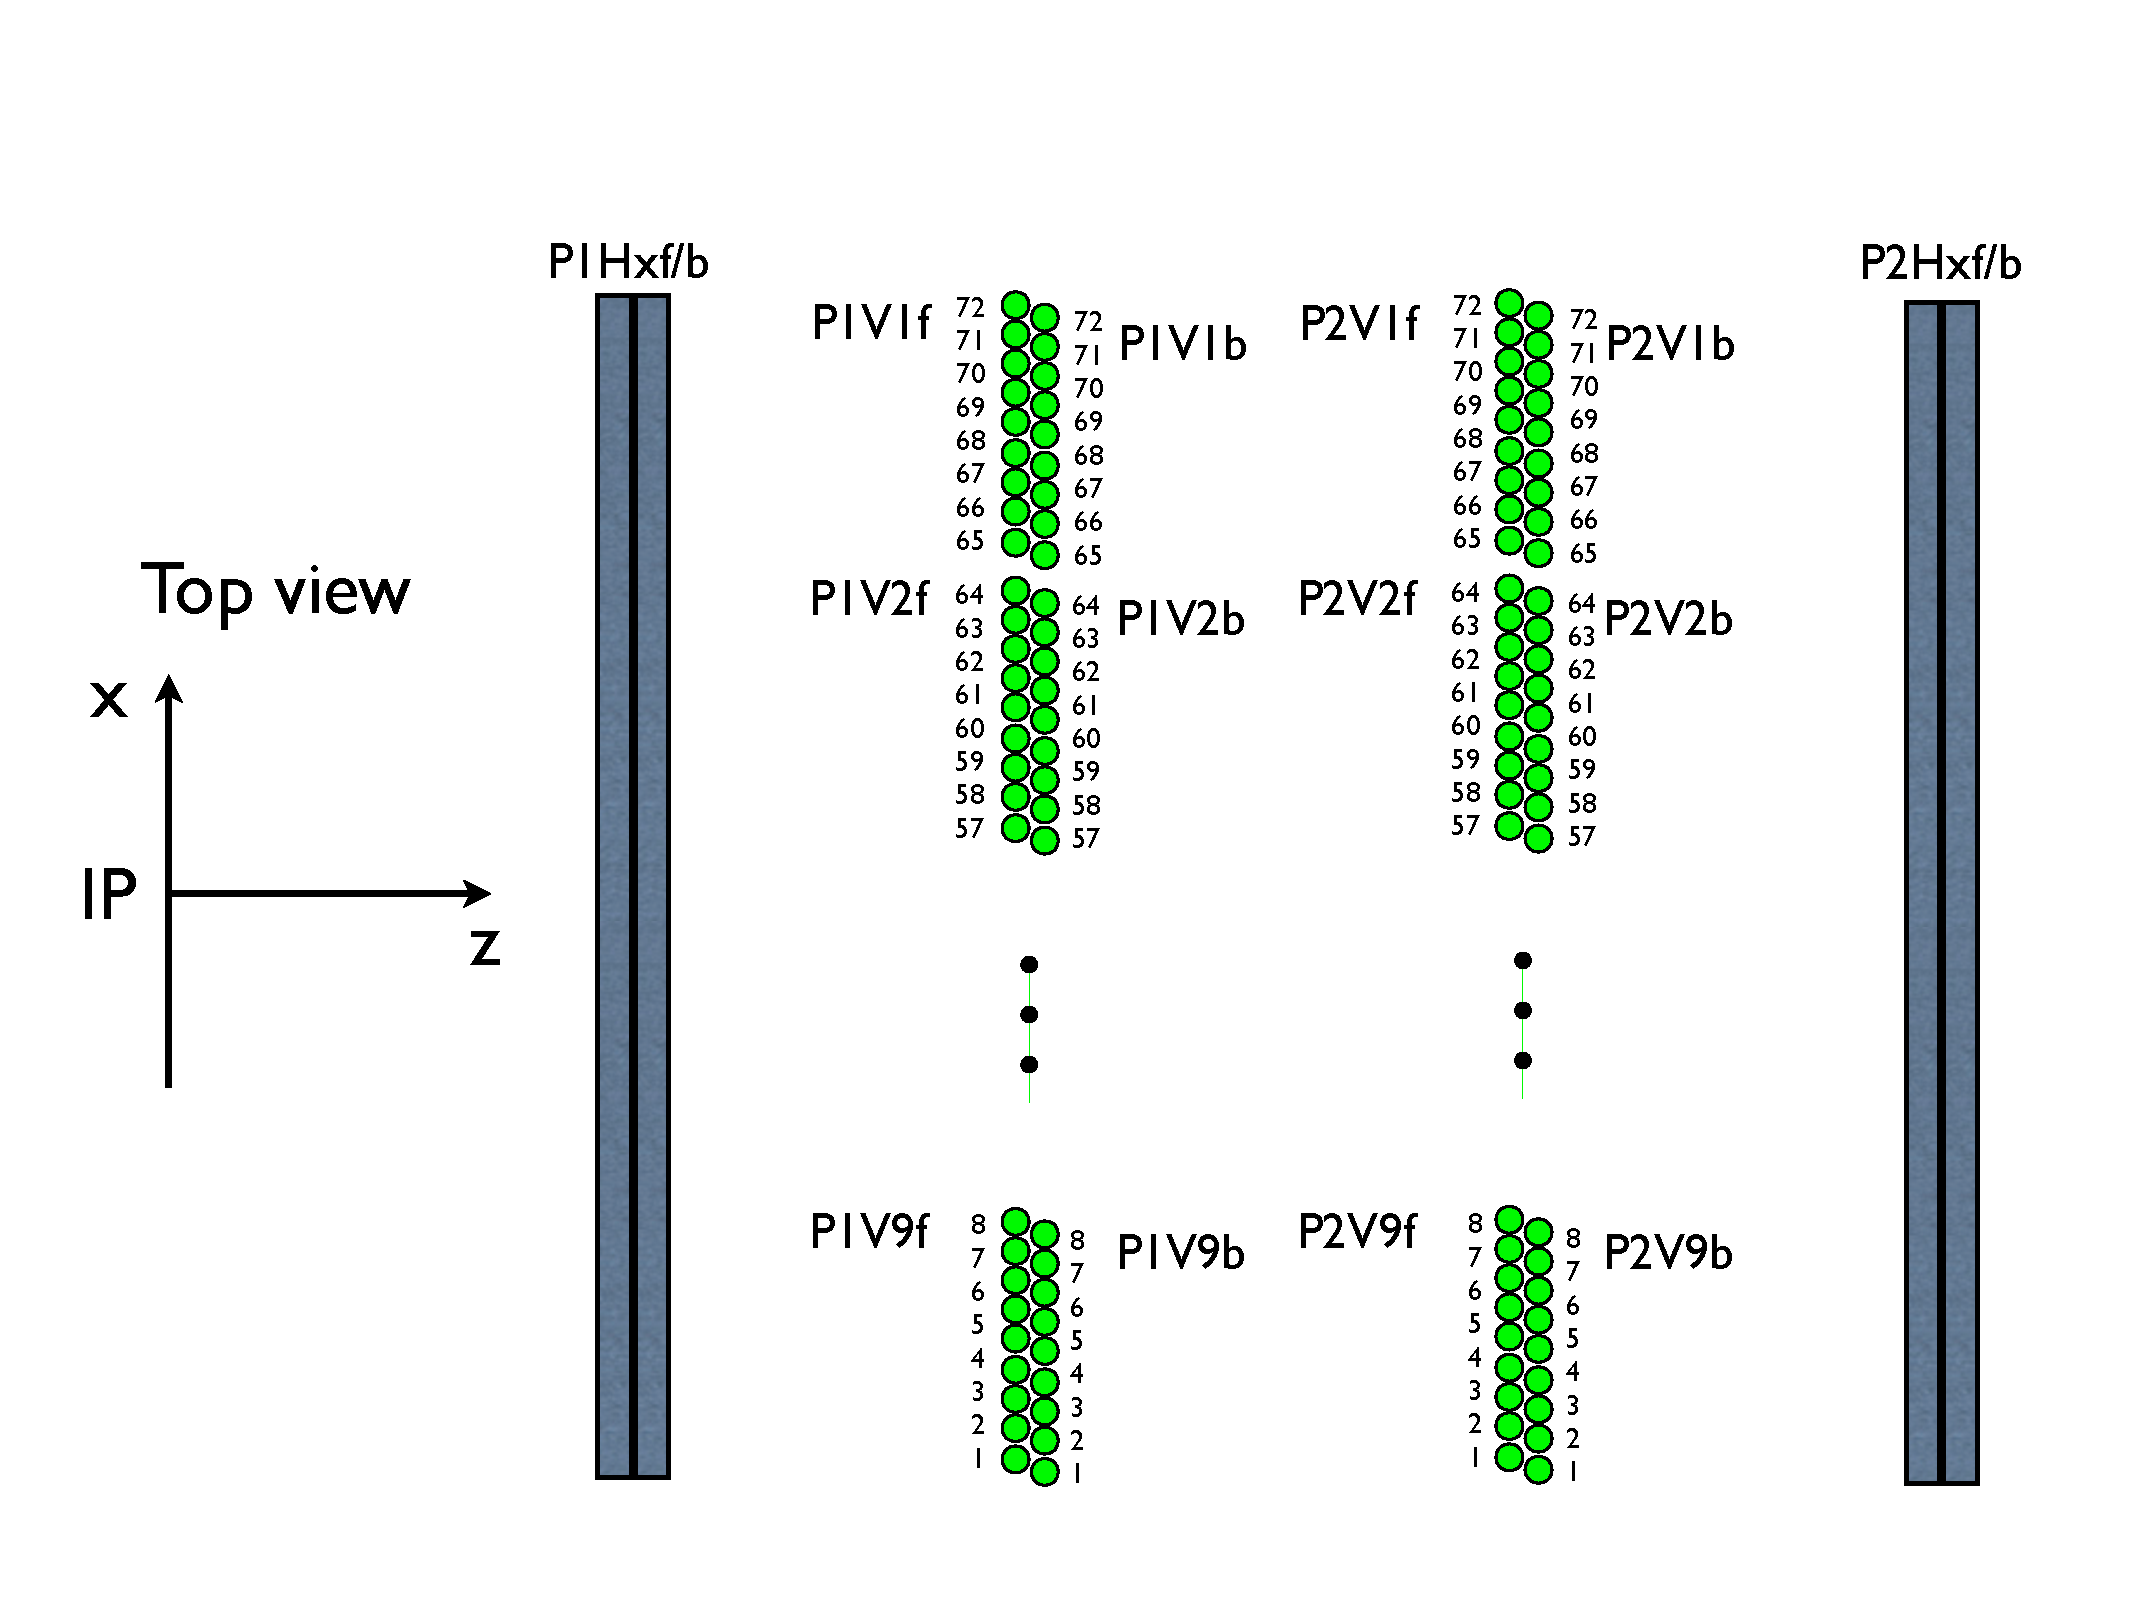
\includegraphics[width=0.9\linewidth]{proptubeview_xz}
	\end{subfigure}
	\begin{subfigure}{0.45\linewidth}
		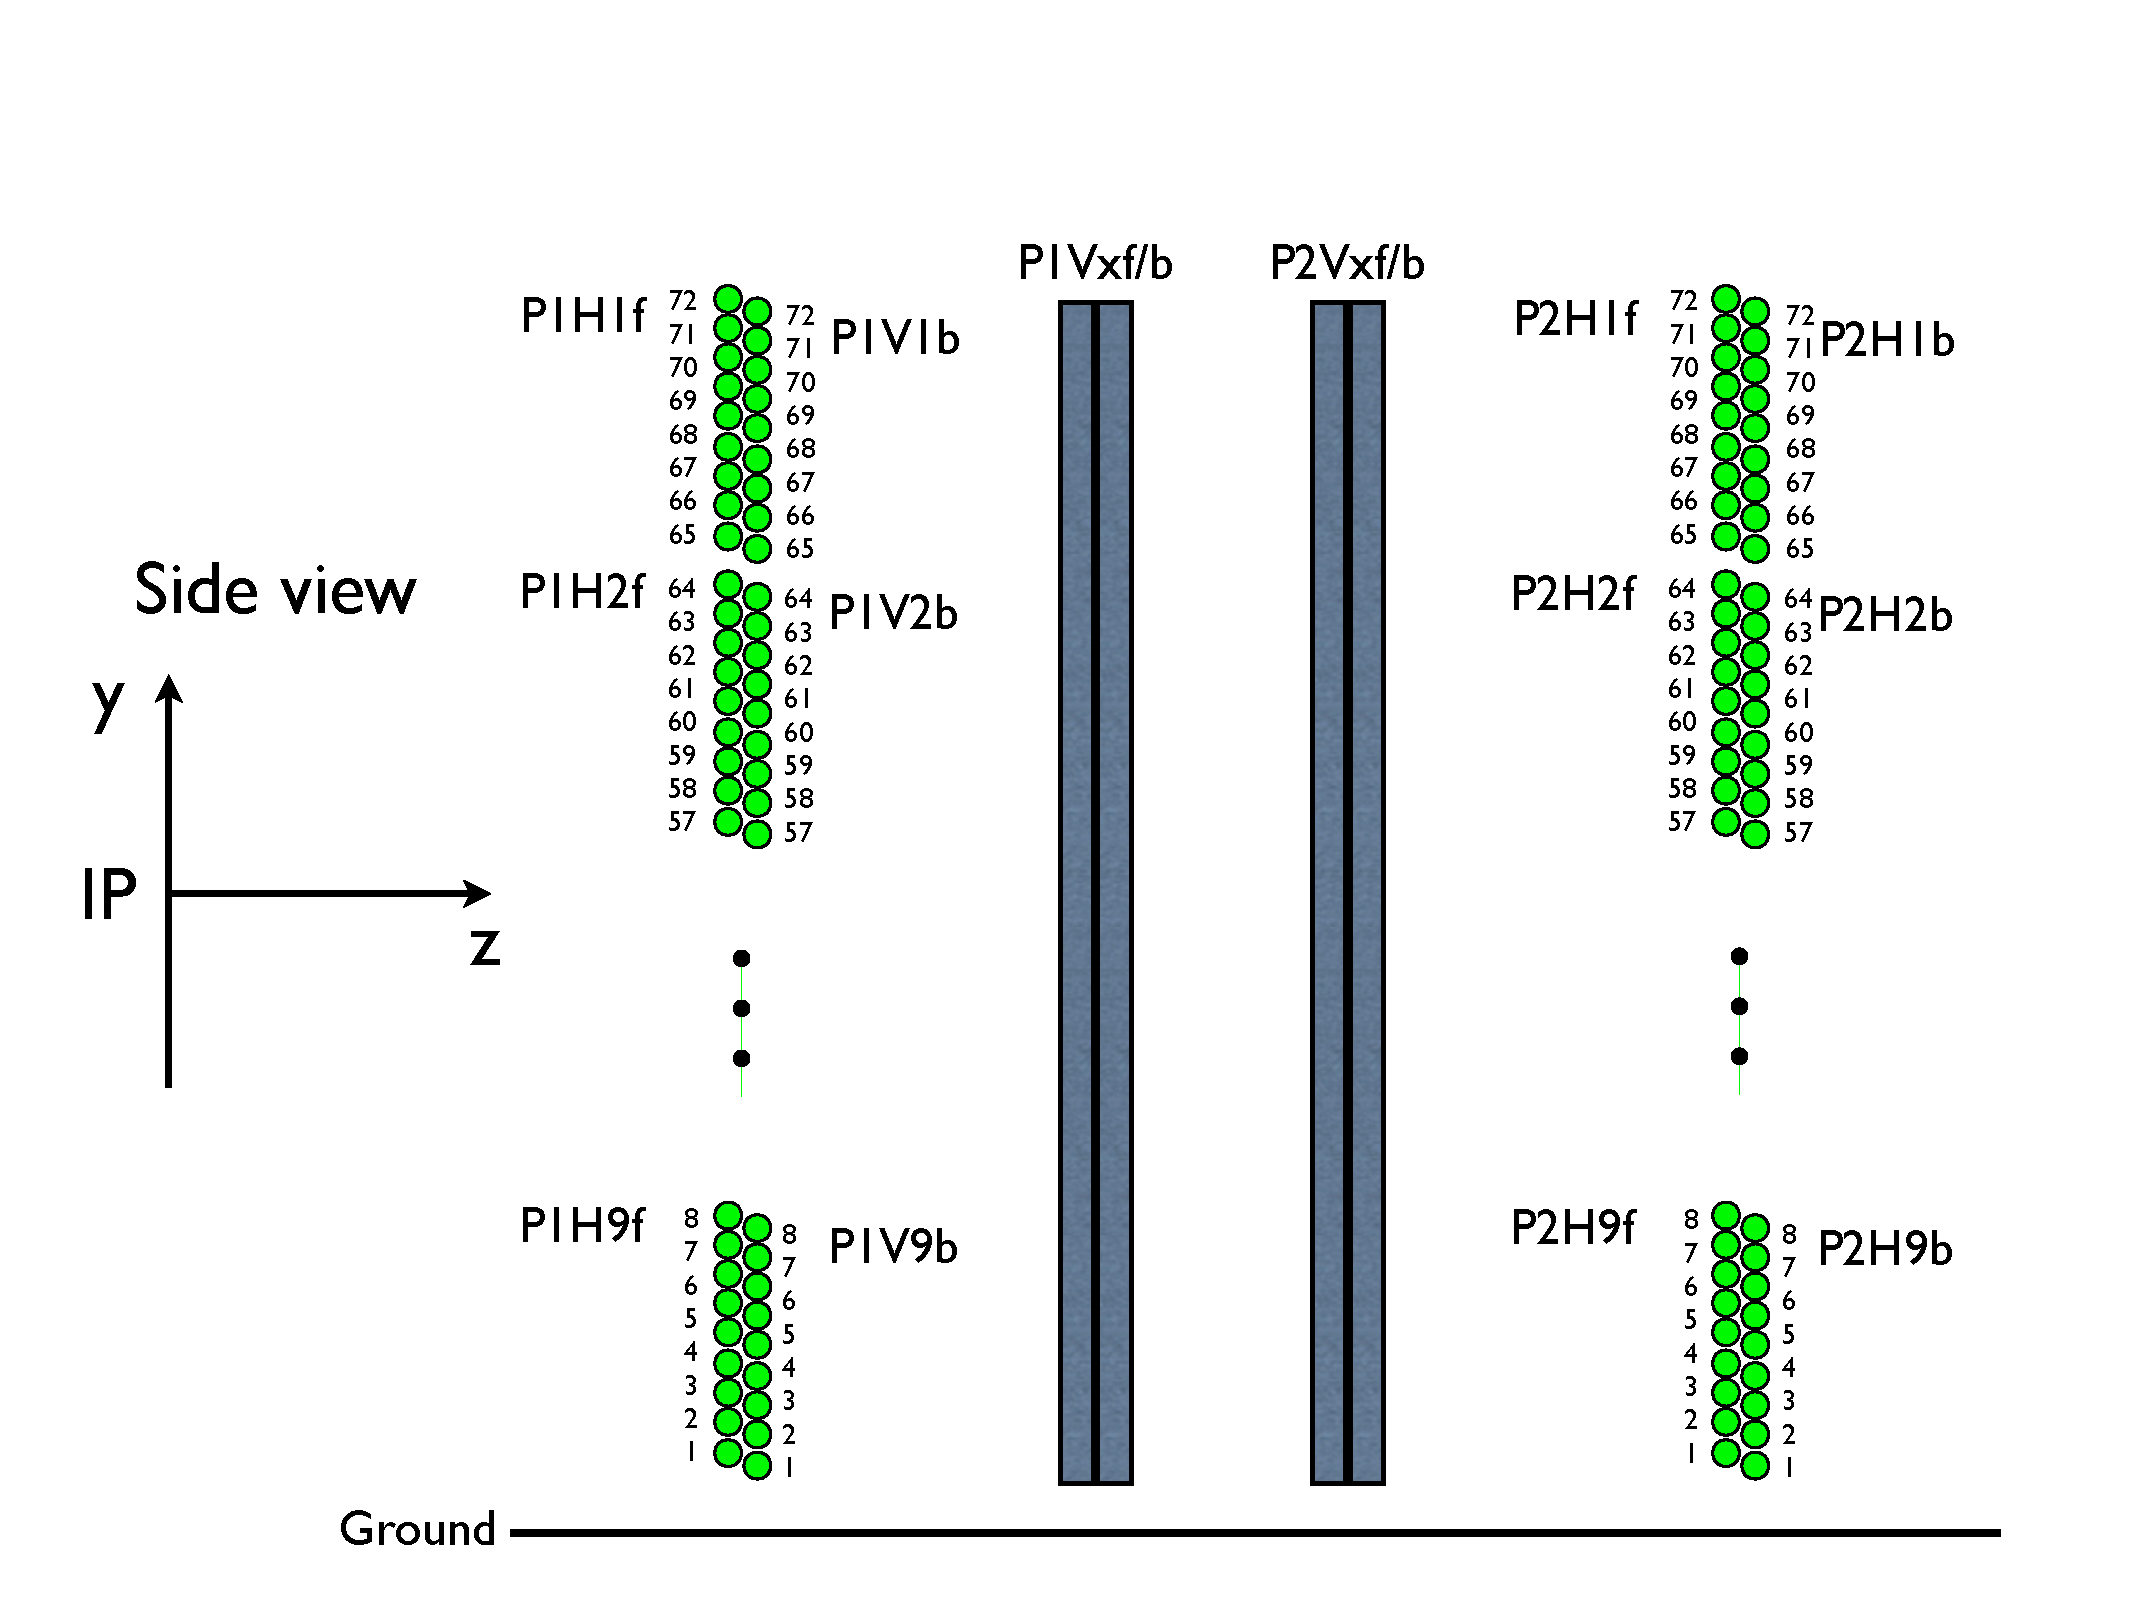
\includegraphics[width=0.9\linewidth]{proptubeview_yz}
	\end{subfigure}
	\caption{XZ (left) and YZ (left) view of the proportional tube at station 4.}
	\label{fig:prop}
\end{figure}
A typical high energy muons would traverse two proportional tubes in each planes.
For muon identification, 8 hits from 4 planes are required, and the hits
should also be pointing back at the target.

\section{Trigger System}
The SeaQuest trigger uses discriminated signals from the hodoscope counters.
Two separate trigger systems are used in SeaQuest, NIM-based and FPGA-based.
The FPGA trigger system is the main trigger system. It utilizes 9 CAEN
v1495 VME modules, Altera EP1C20F400C6 FPGA (Field Programmable Gate Array)
modules. The 9 modules are separated into three levels from level 0 to level
2, as illustrated in \cref{fig:trigger}.
Four FPGA modules form the level 0, with one module for each hodoscope
``quadrant'' (upper bend plane, lower bend plane, upper nonbend plane and
lower nonbend plane). During data taking, level 0 simply passes the input signal
to level 1. The level 0 can also act as a pulser for diagnostic purpose.
At level 1, four FPGA modules are used to search for four-hit track
candidates in each quadrant and compared with a preselected list of hit
patterns, known as trigger roads. The list of trigger roads (known as roadset)
are generated by studying the path of muons from Monte Carlo simulations, with
the goal of persevering signal rates while suppressing backgrounds.
The level 2 consists of a single module, and forms
a trigger decision based on types of track candidates found at level 1. During
SeaQuest data taking, there are five output triggers, as listed in \cref{tab:FPGA}.
During SeaQuest, only x-measuring (bend plane) hodoscopes are used in making
trigger decisions.
\begin{figure}
	\centering
	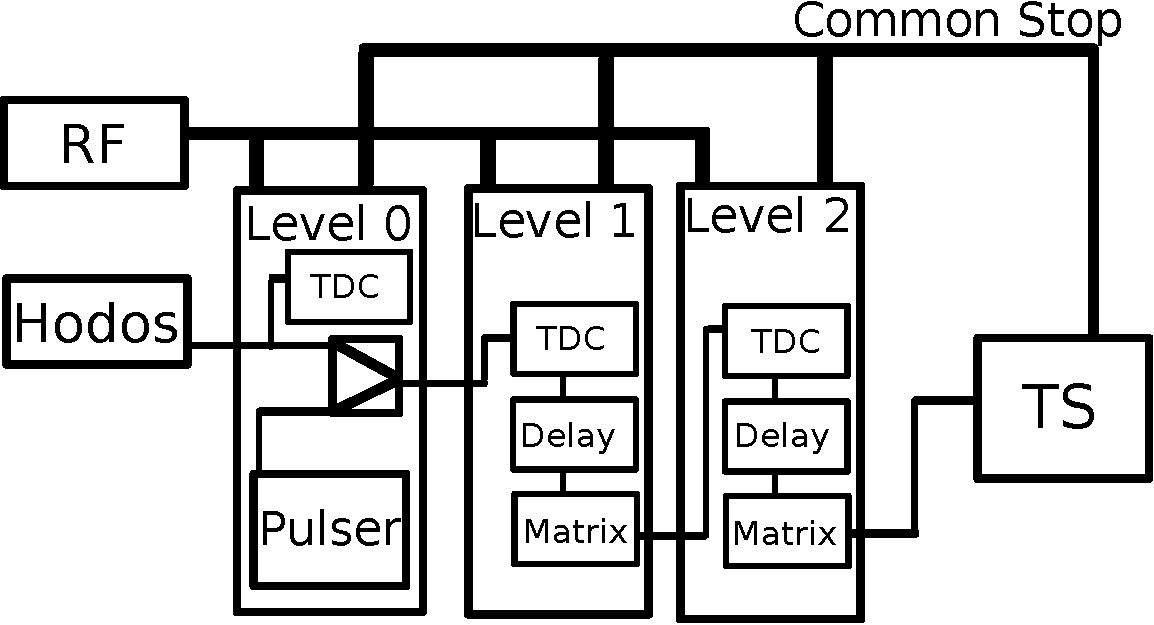
\includegraphics[width=0.5\linewidth]{trigger_schematic}
	\caption{The schematic of the FPGA trigger hardware}
	\label{fig:trigger}
\end{figure}
\begin{table}[h!]
	\centering
	\caption{The five output trigger of the Level 2 trigger module.}
	\label{tab:FPGA}
	\begin{tabular}{lllll}
		Name     & side  & Charge  & $p_x$ Req.         & Notes                     \\ \hline
		Matrix 1 & TB/BT & $+-/-+$ & None               & Main physics trigger      \\
		Matrix 2 & TT/BB & $+-/-+$ & None               & Same-side trigger         \\
		Matrix 3 & TB/BT & $++/--$ & None               & Like-charge trigger       \\
		Matrix 4 & T/B   & $+/-$   & None               & Single muon trigger       \\
		Matrix 5 & T/B   & $+/-$   & $p_x>\SI{3}{\GeV}$ & High-$p_T$ single trigger \\ \hline
	\end{tabular}
\end{table}

The NIM trigger utilizes Nuclear Instrumentation Modules (NIM) to form the trigger
logic. This system is mostly used for debugging and monitoring purpose.
During data taking, two types of NIM trigger are used, known as NIM-1
and NIM-3. The NIM-1 trigger is a coincidence of the y-measuring hodoscope hits
from all 4 stations. This trigger is mainly used for studying the efficiency
of the x-measuring hodoscope, which is important for understanding the performance
of the FPGA trigger system. The second NIM trigger, NIM-3, is also known as a
pulser trigger. It triggers on the coincidence of two clocks, a \SI{7.5}{\kHz}
clock generated by a gate generator and the \SI{53.1}{\MHz} Main Injector
RF clock. The NIM-3 trigger is used to understand the intensity profile of the
beam and the background hits in the spectrometer. The hits from NIM-3 trigger
are also used in the Monte Carlo simulation to understand the rate dependence
of the reconstruction. This will be discussed further in \cref{M-sec:MC}.

\section{Data Acquisition, Decoding and Storage}
The data acquisition for SeaQuest is divided into three separate subsystem, namely
the ``Event DAQ'', ``Scaler DAQ'' and ``Beam DAQ''.

\subsection{Event DAQ}
The Event DAQ records the event-by-event hit information and the trigger timing.
It uses the VME-based ``CODA''~\cite{CODA} system developed by Thomas Jefferson National Accelerator
Facility. This system uses 14 VME crates and can read out different detectors in parallel.
Each VME crate contains a board processor, a trigger interface and a number of TDCs.
Each TDC will read out the hit information from each detector and will be read out by the processor.
There is also a trigger supervisor crate.

The trigger supervisor receives the trigger signals from the trigger matrix and NIM triggers. The trigger supervisor
can receive up to 12 different input triggers. The first 5 bits are used by the FPGA triggers
and the next 3 bits are used by the NIM trigger (NIM-1 to NIM-3). The last 3 bits
are used by BOS (Beginning of Spill), EOS (End of Spill) and flush events.
The trigger supervisor can also prescale the first 8 triggers, such that the high rate triggers can be suppressed.

When the trigger supervisor receives a trigger, it generates a common stop signal, which is fanned out
to the trigger interface in each VME crate. The trigger interface then instructs the processor to readout the TDCs
and send the hit information back to the DAQ host over gigabit Ethernet. The trigger interface then
reports back the to trigger supervisor once the crate has completed the readout. The trigger supervisor can process
a new trigger after all trigger interface has reported back. The trigger supervisor would also send a trigger to QIE,
which allows it to record beam intensity of the 16 RF buckets before and after the trigger.

The deadtime of this system is approximately \SI{150}{\micro\second}. This is primary
dominated by the time required to readout all the TDCs in a single crate. Even though
each detector channel is readout in parallel, the TDCs are read out sequentially
and each hit would take \SI{\sim 4}{\micro\second} to readout. Therefore, high occupancy
events would cause a longer deadtime.

Between Run 5 and Run 6, an upgrade was preformed to the Event DAQ \cite{Kun-1724}.
Taking advantage of the beam structure, where the beam is only on for \SI{4}{\s} every minute,
the hit information can be buffered in the VME during beam-on and only sent to the Event
DAQ host during beam-off. When a hit occurred on a detector,
the timing information is stored on a ring buffer.
When a trigger signal is received by the trigger supervisor,
a common-stop signal is issued to all TDCs. The TDCs will then store the hit information
to an event buffer. Once the spill is over, the readout controller will read the event
buffers on all the TDCs and send the hit information back to the DAQ host.
This design reduces the deadtime from $150 -200\unit{\micro\second}$ per event to a fixed $28\unit{\micro\second}$.

\subsection{Scaler DAQ}
The Scaler DAQ operates independently of the Event DAQ.
It is alive regardless of the status of the Event DAQ.
It is designed to monitor the spectrometer and trigger,
providing fast diagnostic data while the experiment is running. Like the Event DAQ,
it utilizes the ``CODA'' system. It consist of a single VME crate with four scaler
cards. The Scaler DAQ is triggered by a \SI{7.5}{\kilo\hertz} clock and the beam
spill signal. It uses 3 VME scale 32 modules to record data such as number of triggers
and hodoscope rates. The Scaler DAQ data are processed in real time and displayed
on a monitor in the SeaQuest Control room.

\subsection{Beam DAQ}
\label{subsec:beamDAQ}
The Beam DAQ aims to provide the instantaneous beam intensity with the Cerenkov counter.
The signal from the Cerenkov counter is sent to a Fermilab-designed QIE module.
This custom module is synced to Main Injector RF clock and it reads out the Cerenkov
counter every 18.8 ns clock cycle. The Beam DAQ host then reads out this custom module
after each spill to provide the integrated beam intensity for the entire spill.
The Beam DAQ is also linked with the Event DAQ so it can calculate the integrated spill
during trigger dead time and the 16 buckets before and after each trigger.
The Beam DAQ will also monitor the instantaneous beam intensity and inhibit the trigger if the
intensity is above a certain threshold. The Beam DAQ will record the integrated intensity
while inhibit is asserted at trigger logic.




\subsection{Slow Controls}
Slow Controls refer to several script, which utilizing the standard Experimental Physics and Industrial Control
System (EPICS)~\cite{dalesio1994}, to synchronize the different DAQ data streams, monitor the various systems,
and to record process variables at a timescale of a spill or longer.

Each DAQ system writes its output to separate files, in order to synchronize the different data streams,
a script is used to manage a master spill ID and insert the spill ID into the different data streams.
This allows the decoder to reassemble the data offline. The spill ID is also written to the EPICS server.
Another slow control program is also connected to the Fermilab accelerator control network (ACNET).
This allows us to record the current to the different spectrometer magnets, target position
and status of the target cryogenic system. A multi-channel digital meter is also used to record
the environmental conditions such as temperature and humidity inside the experimental hall.

\subsection{Decoder and Storage}
Typically, each run of physical data taking lasts about an hour. The file size is typically
several \unit{\giga\byte}s. The data files from all the DAQ systems and slow control system
are stored locally in a disk array located in the SeaQuest control room. The data from DAQ
is also backed up on tape storage provided by Fermilab computing division.

The Event DAQ and Scaler DAQ write their output in a CODA specific binary format. The Event
DAQ file contains the TDC information from each detector of each triggered events. The instantaneous
beam intensity around the triggering bucket from the BeamDAQ is also attached in the Event DAQ file.
These raw data files are processed by a custom program called ``decoder", which coverts the
CODA specific format into a ROOT based format. These information will also be uploaded to a SQL
server.

\ifSubfilesClassLoaded{ \printbibliography[heading=bibintoc,title={References}]}{}
\end{document}
